\section{Reference Frames}
\label{reference_frames}

In this section, we review the concepts of coordinate frame transformations. 
We will start with 2D transformations and then see more on 3D transformations. 

The coordinate frames we use are right-handed frames by convention, and we'll use a few standard coordinate frames.
The global world or inertial coordinate frame, is a fixed reference frame attached to the earth. Often, we'll represent this coordinate frame as East North Up, ENU, relative to a reference point nearby. Or Earth-Centered Earth Fixed, ECEF, as is used in GNSS systems.

\begin{figure}[!htb]
\begin{center}
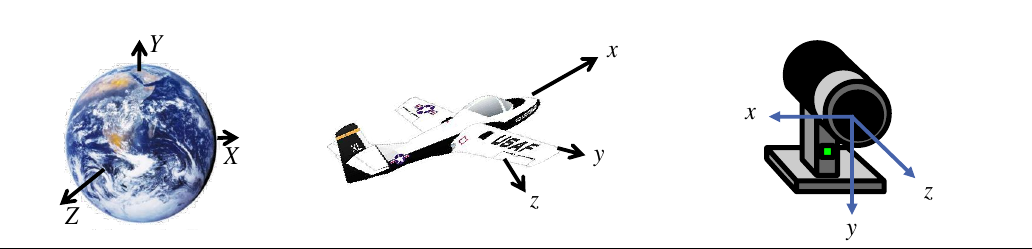
\includegraphics[scale=0.290]{img/coordinate_transforms/coordinate_framew.jpeg}
\end{center}
\caption{Schematic of coordinate frames.}
\label{coordinate_framew}
\end{figure}


The next frame we'll talk about is the body frame, which is placed in some key location on the body of the vehicle. For example, the center of gravity (CoG) of a vehicle or the center point of the rear axle. This frame is moving and rotating with respect to the fixed inertial frame as the vehicle moves about.

Finally, the sensor frame is a coordinate frame which attaches to each sensor describing the coordinates used for the sensor output. In many robotics applications, we need to attach several coordinates to a moving system and also represent elements from these frames in the inertial frame. To do this, we need to transform variables from one coordinate frame to the other. For example, from the body frame to the inertial. Even a simple two wheeled robot with a single sensor has three such frames to consider, while the self-driving car can have dozens.

To maintain a consistent representation of sensor data for perception, we need to be able to transform information between coordinate frames. 
Let's take a look at a simple transformation example for a velocity vector of a car.

\begin{figure}[!htb]
\begin{center}
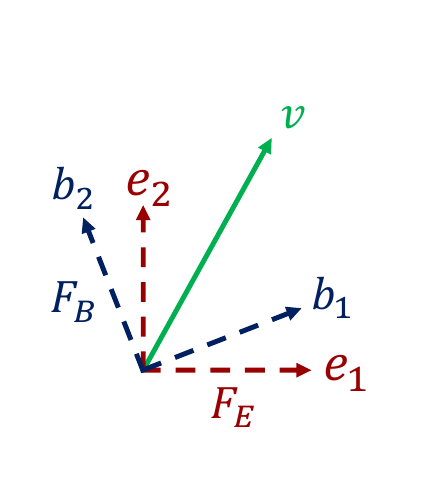
\includegraphics[scale=0.290]{img/coordinate_transforms/vector_rotation.jpeg}
\end{center}
\caption{Schematic of vector rotation.}
\label{vector_rotation}
\end{figure}


Generally, kinematic variables such as velocity are represented in the form of a vector, with both magnitude and direction. In figure \ref{vector_rotation}, the vector $v$ is presented with a green arrow in a two-dimensional coordinate frame. We have two coordinate frames displayed here. The body frame, defined by axes $b_1$ and $b_2$, and the inertial frame defined by axes $e_1$ and $e_2$, both in the 2D plane. 

Let's assume the two coordinate frames; frame $e$ and frame $b$, have the same fixed origin. But frame $b$ is rotated by some angle $\theta$ relative to frame $e$. We can then define the rotational matrices $C_{EB}$, which transforms vectors from the frame $b$ to the frame $e$ and $C_{BE}$ which projects the frame $e$ onto frame $b$ using the angle $\theta$ as shown.

\begin{equation}
C_{EB} = 
\begin{bmatrix}
 \cos(\theta) & \sin(\theta) \\
 -\sin(\theta) & \cos(\theta) 
\end{bmatrix}, ~~
C_{BE} =
\begin{bmatrix}
 \cos(\theta) & -\sin(\theta) \\
 \sin(\theta) & \cos(\theta)
\end{bmatrix} 
\end{equation}

\begin{figure}[!htb]
\begin{center}
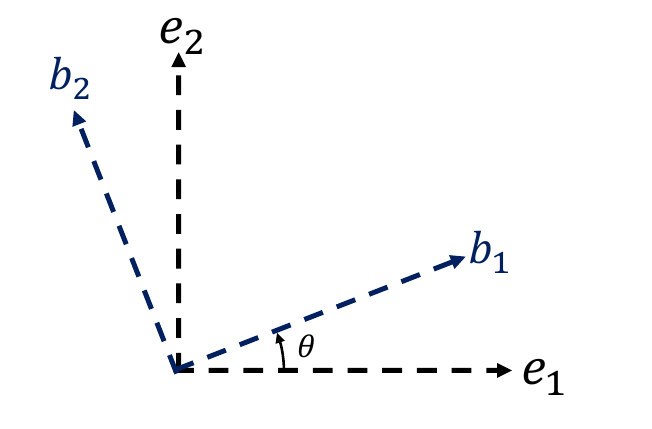
\includegraphics[scale=0.290]{img/coordinate_transforms/theta_angle.jpeg}
\end{center}
\caption{Rotation angle $\theta$.}
\label{theta_angle}
\end{figure}


Now, let's extend our example to include a translation. Here, we see a two-wheeled robot and we'd like to represent the position of a point $P$ 
observed by the robot in the robot body frame $b$, with respect to the inertial frame $e$. 
The position of the robot with respect to the inertial frame is $(x, y)$, and the orientation of the robot once again is $\theta$.


\begin{figure}[!htb]
\begin{center}
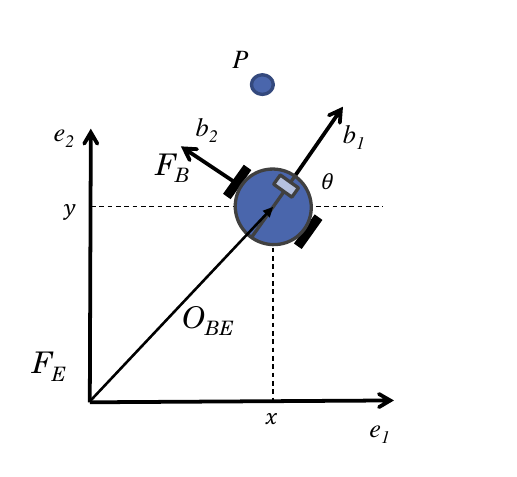
\includegraphics[scale=0.290]{img/coordinate_transforms/robot_orientation.jpeg}
\end{center}
\caption{Rotation angle $\theta$.}
\label{robot_orientation}
\end{figure}

The following equations relate the location of point $P$ in the body coordinates $P_B$ and the inertial frame $P_E$. 
Note that in general to transform one point from one coordinate to the other coordinate frame, body to inertial and vice versa, requires two terms. The translation of the origin $O_{BE}$ and $O_{EB}$ in this case, and the rotation of the axis $C_{EB}$ and $C_{BE}$. Finally, we can summarize the transformation between two coordinate frames using homogeneous coordinates, which lead to a compact matrix multiplication to apply the transformation. 

\begin{equation}
P_B = C_{EB}(\theta)P_E + O_{EB}
\end{equation}

where $O_{EB}$ is the translation term expressed in body frame. Similarly,

\begin{equation}
P_E = C_{BE}(\theta)P_B + O_{BE}
\end{equation}


We extend our location vector to include $(x, y)$, and one and can then transform from body to inertial coordinates using $P$ inertial is $C_{EB}$ and $O_{EB}$ times $P$ in the body frame. 


